\documentclass{article}

% Language setting
% Replace `english' with e.g. `spanish' to change the document language
\usepackage[english]{babel}
\usepackage[utf8]{inputenc} % für Umlaute
\usepackage{fontenc}

% Set page size and margins
% Replace `letterpaper' with`a4paper' for UK/EU standard size
\usepackage[a4paper,top=2cm,bottom=2cm,left=3cm,right=3cm,marginparwidth=1.75cm]{geometry}

%%%% ---- Useful packages

%%% --- Figures and Graphics
\usepackage{graphicx}
\usepackage{subcaption}
\usepackage{tikz}

%%% --- Colors
\usepackage[]{xcolor}

%%% --- Tabulars
\usepackage{booktabs}

%%% --- Mathematics
\usepackage{amsmath,amsfonts,amssymb,amsthm,mathtools}
\usepackage{bm} % bold mathematics
\usepackage{bbm} % for blackboard 1
\usepackage[linesnumbered,lined,algo2e,figure,boxed]{algorithm2e}
\usepackage[short]{optidef} % for aligning linear programs

%%% --- Other
\usepackage[colorlinks=true, allcolors=blue]{hyperref}
%\usepackage[hidelinks]{hyperref}
\usepackage[style=authoryear,backend=bibtex]{biblatex}
%\addbibresource{library.bib}
\usepackage{csquotes}
\usepackage[shortcuts]{extdash} % For Hyphens in English
%\usepackage{acro}
% \DeclareAcronym{pdf}{short=PDF, long={probability distribution function}}

%%% --- Commenting, Todonotes
\usepackage{comment, todonotes}
\newcommand{\ar}{$\rightarrow$}
\presetkeys{todonotes}{backgroundcolor=yellow!30, bordercolor=yellow!50, linecolor=yellow!50, figwidth=\textwidth}{}
\newcommand{\hl}[1]{\textcolor{Aquamarine}{#1}}

%%%% ---- Own Commands
%%% --- Theorem Settings
\theoremstyle{plain}% Theorem-like structures provided by amsthm.sty
\newtheorem{theorem}{Theorem}
\newtheorem{exa}{Example}
\newtheorem{rem}{Remark}
\newtheorem{proposition}{Proposition}
\newtheorem{lemma}{Lemma}
\newtheorem{corollary}{Corollary}

\theoremstyle{definition}
\newtheorem{definition}{Definition}
\newtheorem{remark}{Remark}
\newtheorem{example}{Example}

%%% --- Math Commands

\newcommand{\lag}[1][l]{\Delta_{#1}}
\DeclarePairedDelimiter{\abs}\lvert\rvert
\DeclareMathOperator{\sign}{sign}
\newcommand{\tmax}{\bar{t}}
\newcommand{\ind}{\mathbbm{1}}

%%% --- Other Commands
\renewcommand{\arraystretch}{1.2}

%%% --- ToDo List
\usepackage{enumitem}
\newlist{todolist}{itemize}{2}
\setlist[todolist]{label=$\square$}
\usepackage{pifont}
\newcommand{\cmark}{\ding{51}}%
\newcommand{\xmark}{\ding{55}}%
\newcommand{\done}{\rlap{$\square$}{\raisebox{2pt}{\large\hspace{1pt}\cmark}}%
\hspace{-2.5pt}}
\newcommand{\wontfix}{\rlap{$\square$}{\large\hspace{1pt}\xmark}}

\title{Trending in Nowcasting}
\author{Oliver Grothe, Bolin Liu, Jonas Rieger}

\begin{document}
\maketitle

%\begin{abstract}
%Your abstract.
%\end{abstract}

\section{ToDos}


\begin{todolist}
\item Differenz gegen was? (alte Realisierung oder alter Nowcast) "Problem": Nowcaster, der schon lange far off liegt messe ich gegen das falsche? Wie lange weiß er den heutigen Wert schon? Gegeben, seinem Wissenstand: Ab wo er es kennt gegen $y$, davor gegen $x$.
\item was glaubt er heute - (was glaubt er heute von gestern?)
\item "Irrelevante Änderung" statt Rauschen
\item Berechnung $\sigma$: Theoretisch aus Daten vs. Gefilterten Daten; Aus Wendepunkten; einfach mal durchlaufen lassen
\item Rauschen-Schätzer berechnen für neue Deltas; verschiedene Sigmas
\item Sigma bestimmen: einmal aus Plot von $k$ über verschiedene $\sigma$, einmal über Gefilterte vs. reale Daten
\item $\varepsilon$ für beide Komponenten oder nur für eine? Unterschiedliche $\sigma$ für $X$ und $Y$? $\sigma$ nur auf $Y$ anwenden.
\end{todolist}


The evaluation of measurement, prediction, and forecasting methods becomes increasingly important and sophisticated as technologies and data availability enable their application in more and more fields. 
Conventionally, methods are evaluated using distance measures of local differences between predictions (or measurements) and target values. 
These measures do not consider whether the right direction of change is predicted or measured.
The information about whether an increase or decrease is predicted correctly is crucial when making decisions based on the estimator's prediction results. 
In the following, we provide a more specific overview of the characteristics and current evaluation schemes of the three application fields, forecasting, nowcasting, and measurement, and highlight why trending evaluation is highly relevant in the respective fields.

The above-described trending idea is of fundamental interest for evaluating and comparing forecasting methods. 
Forecasting methods predict the future based on historical data, patterns, and exogenous factors. 
The forecast is computed based on the current value of the quantity of interest and an estimate of the development until the target time.
A forecast's trending is perfectly consistent with the actual development of the target value if the actual change in the target value over this period matches the forecast change. 
In the current practice, a forecasting method is usually evaluated in terms of its prediction accuracy, measuring the deviation of the prediction from the actual outcome of the target variable. 
Popular measures are scale-dependent measures such as the \ac{rmse}, measures based on percentage errors such as the root mean squared percentage error, or probabilistic scoring rules \textcite[see the review in][]{hyndman2006another}. 
These typical measures are based on the absolute difference between the prediction and the true values, locally or globally. 
They are not capable of assessing the trending ability discussed above.

Methodologically evolved from forecasting, nowcasting methods focus on predictions for the present, the immediate future, and the recent past \parencite{banbura2013now} and are now widely used in fields such as economics and medicine \parencite{bok2018macroeconomic, Wolffram2023}.
Nowcasting has its origins in meteorology, and the methods were initially developed to describe the current state of the weather in detail and to predict the expected change on a time scale of a few hours \parencite{browning1989nowcasting,schmid2019nowcasting}. 
In economics, nowcasting is used to predict statistics on the current economic situation, for example, the gross domestic product, which is collected with low frequency and is available with a considerable time delay \parencite{banbura2013now}.
In medicine, epidemic nowcasting assesses the current situation during an ongoing epidemic, considering the main pathogenic, epidemiological, clinical, and socio-behavioral factors \parencite{wu2021nowcasting}. 
Nowcasting methods use high-frequency indicators related to the target variable and estimate the value of a target variable for a specific time based on current preliminary measurements, which are finalized with a considerable time delay. 
Thus, the nowcasts can produce early and ongoing estimates for the target variable during the relevant period \parencite{castle2017forecasting}. 
For example, the nowcasting method can correct the daily COVID case numbers for events that have occurred but have not yet been reported \parencite{gunther2021nowcasting}. 
Like forecasts, nowcasts are often evaluated and compared in the literature based on performance measures such as the \ac{rmse} \parencite{gunther2021nowcasting} or probabilistic scoring rules \parencite{Wolffram2023}. 
The aspect of trending ability is not considered in the literature to the best of our knowledge. 
However, trending evaluation adds valuable information on the methods' capability of predicting the development of the target variable, for example, the number of cases of an epidemic.
The epidemic's development, in turn, can be the foundation of decisions on introducing or canceling policy measures. 

Measurement aims to obtain accurate and reliable data about the current state of a system. 

A parameter or variable can be measured regularly over a certain period to evaluate the system's development.
When introducing new measurement methods, they are evaluated against current measurement techniques, called the gold standard, by measuring the same quantity in different settings, such as individuals or environments.
Various indices, such as the interclass correlation coefficient or Lin's concordance correlation, have been proposed to check the reproducibility of the measurement or to compare different measurement methods \parencite{lawrence1989concordance,koo2016guideline} in addition to paired t-tests to determine systematic differences between two measurement series \parencite{watson2010method}. 
Furthermore, graphical tools were developed, such as the Bland-Altman diagram, visualizing the differences between the methods in relation to their mean value \parencite{bland1986statistical}. 
Trending considerations, that is, the consistency of the test methods development with the gold standard, is a field of active research in the last years \parencite{Saugel2015,saugel2018error,hiraishi2021concordance}. 
In this paper, we build upon the existing methods and extend them with new functionality.

As outlined above, trending evaluation is crucial for measurements, predictions, and forecasts. 
However, regardless of the application area, most conventional method comparisons and assessments consider local absolute deviations without assessing whether the correct direction of change is being predicted or measured. 
In this paper, we develop trending evaluation methods that complement current evaluation measures with trending measurements.

The main contributions of this paper are manifold.
\begin{itemize}
\item We formalize trending and present different variants of trending measures that consider either noiseless data or data with noise and small non-informative changes.
\item We introduce the conditional trending plot, a new graphical method for assessing local trending behavior, and review bootstrap methods for calculating confidence intervals.
\item We extend the concept of trending to probabilistic predictions.
\item We apply trending evaluation to three applications: Measurement, nowcasting, and forecasting data. 
\item We provide a ready-to-use code for trending evaluation. The code and the source code to replicate the results of our study are available at ... .
\end{itemize}

The remainder of this paper is structured as follows. 
Section \ref{sec:trending} formalizes trending and investigates several extensions, such as noise-aware methods, confidence intervals, and probabilistic forecasts and nowcasts. 
In particular, we introduce a new graphical method for evaluating trending, the conditional trending plot, which can represent the simultaneous evaluation of different intervals and asymmetries. 
In Section \ref{sec:application}, we show the results of applying our method to several practical examples from measurement, forecasting, and nowcasting. 
We conclude the paper in Section~\ref{sec:conclusion}.


\section{Notation}
\begin{itemize}
  \item Sei $T = \{1, 2, \dots\}$ die Zeitindexmenge, wobei für jeden Zeitpunkt $t \in T$ eine Realisierung vorliegt (die ggf. im Nachhinein veröffentlicht wird).
  \item Sei $(Y_t)_{t \in T}$ die Zeitreihe der Realisierungen, dabei steht $t$ für den Zeitpunkt, auf den sich der Wert bezieht, nicht den Veröffentlichungszeitpunkt.
  \item Sei $K = \{1, 2, \dots\}$ die Menge der Nowcaster.
	\begin{itemize}
	  \item Sei $X_{t \lvert \tau}^k (k \in K, t \in T, \tau \in T_t^k)$ der Nowcast von $k$ bezüglich des Zeitpunktes $t$, der am Zeitpunkt $\tau$ \textbf{veröffentlicht} wird (oder: berechnet / dessen Informationen sich auf Zeitpunkt $\tau$ beziehen).
	  \item Sei $g: \mathbb{R}^{\lvert T_t^k \lvert} \rightarrow \mathbb{R}$ eine Aggregationsfunktion, die alle Nowcasts bezüglich eines Zeitpunkts zu einem Nowcast zusammenfasst ($X_t^k \coloneqq g((X_{t \lvert \tau}^k)_{\tau \in T_t^k})$). Falls jeweils nur ein Nowcast veröffentlich wird, wähle $g(x) = x$.
	  \item Sei $(X_t^k)_{t \in T}$ die Zeitreihe der aggregierten Nowcasts.
	\end{itemize}
  \item Sei $\lag[l]$ der lag-$l$-Operator, der für eine Zeitreihe $(Z_t)_{t \in T}$ definiert wird durch 
		\begin{equation}
			\lag[l]Z_t = Z_{t+l} - Z_t \quad (t \in T)
		\end{equation} 
  \end{itemize}

\begin{figure}
	\centering
\begin{tikzpicture}[scale=2]
\newcommand{\maxaxis}{1.5}
% Draw quadrants with light colors
\fill[green!30] (-\maxaxis,-\maxaxis) rectangle (0,0); % Quadrant B
\fill[red!30] (0,-\maxaxis) rectangle (\maxaxis,0); % Quadrant D
\fill[red!50] (-\maxaxis,0) rectangle (0,\maxaxis); % Quadrant C
\fill[green!50] (0,0) rectangle (\maxaxis,\maxaxis); % Quadrant A

% Quadrant borders
\draw[thick, ->] (-\maxaxis,0) -- (\maxaxis,0); % x-axis
\draw[thick, ->] (0,-\maxaxis) -- (0,\maxaxis); % y-axis
%\draw (0,0) node[below left] {0};
\draw (\maxaxis,\maxaxis) node[below left] {A};
\draw (\maxaxis,-\maxaxis) node[above left] {D};
\draw (-\maxaxis,\maxaxis) node[below right] {C};
\draw (-\maxaxis,-\maxaxis) node[above right] {B};

% Random points
%\foreach \x/\y/\label in {0.6/0.8/z_1, -0.4/0.5/z_2, 0.3/-0.7/z_3, -0.8/-0.2/z_4} {
%  \coordinate (point) at (\x, \y);
%  \fill (point) circle (1.2pt);
%  \node[above right] at (point) {$\label = (\label^x, \label^y)$};
%}

% Axis labels
\draw (\maxaxis,0) node[right] {$\lag y$};
\draw (0,\maxaxis) node[above] {$\lag x$};

\end{tikzpicture}
\caption{Die Quadranten eines 4Q-Plots. In den grünen Quadranten A und B stimmt die Richtung der Veränderung von $\lag x$ und $\lag y$ überein, in den roten C und D nicht.}
\label{fig:quadranten}
\end{figure}


\section{Trending-Problem}


Gegeben seien zwei Zeitreihen $y_1, \dots, y_{\tmax}$ und $x_1, \dots, x_{\tmax}$ aus Realisierungen beziehungsweise Nowcasts zu den Zeitpunkten $1, \dots, \tmax$. 
Hohes Trending liegt vor, wenn der Nowcast die Veränderung der Realisierungen häufig richtig angibt, d.h. der Nowcast höhere Werte angibt, wenn die Realisierung gestiegen ist und niedrigere Werte, wenn sie gefallen ist. 
Mathematisch lässt sich die Wahrscheinlichkeit für eine Entwicklung in die gleiche Richtung bezüglich eines Lags $l$ darstellen als
\begin{equation}
  P((\lag Y) (\lag X) > 0). \label{eq:concordance}
\end{equation}


Eine Möglichkeit, Gleichung \eqref{eq:concordance} zu schätzen, ist
\begin{equation}
  \frac{1}{\tmax - l} \sum_{t = 1}^{\tmax - l} \ind\{{(\lag y_t) (\lag x_t) > 0}\}
\end{equation}

\subsection{Direkte Integration der Rauschen-Betrachtung in die obige Formel}
Dabei wird nicht beachtet, ob Punkte \enquote{mittig} in den Quadranten liegen oder weit am Rand, deswegen könnte das Maß folgendermaßen variiert werden.
Zur einfacheren Notation im Folgenden lassen wir $\lag$ weg.
Wir nehmen an, dass die echten Veränderungen $X$ und $Y$ fehlerbehaftet gemessen werden und nur

\begin{align}
	X_b &= X + \epsilon_X \quad \text{beziehungsweise} \\
	Y_b &= Y + \epsilon_Y 
\end{align}

beobachtet werden können. 
Wir bezeichnen mit $Z_b = (X_b, Y_b)$, $Z = ( X, Y)$ und die Quadranten gemäß Schaubild Abbildung~\ref{fig:quadranten}. 
Wir treffen zwei Annahmen: die Fehler $\epsilon_X$ und $\epsilon_Y$ sind unabhängig und identisch normalverteilt mit Erwartungswert 0 und Varianz $\sigma^2$.
Dann ist die Wahrscheinlichkeit, dass ein Punkt tatsächlich konkordant ist, d.h. $xy > 0$, für gemessene Werte $z_b$
\begin{align*}
	k(z_b) &= P(Z \in A | X_b = x_b, Y_b = y_b) + P(Z \in B | X_b = x_b, Y_b = y_b) \\
	&= (1 - P(Z \in B | X_b = x_b, Y_b = y_b) - P(Z \in C |X_b = x_b, Y_b = y_b) \\
        &\phantom{==} - P(Z \in D |X_b = x_b, Y_b = y_b)) + P(Z \in B | X_b = x_b, Y_b = y_b) \\
	&= 1 - 2 P(Z \in C | X_b = x_b, Y_b = y_b) - 2 P(Z \in D | X_b = x_b, Y_b = y_b) \\
	&= 1 - 2 P(Y \leq 0 | X_b = x_b, Y_b = y_b) - 2 P(X \leq 0 | X_b = x_b, Y_b = y_b) + 4 P(Y \leq 0, X \leq 0| z_b) \\
	&= 1 - 2 P(y_b - \epsilon_Y \leq 0) - 2 P(x_b - \epsilon_X \leq 0) + 4 P(y_b - \epsilon_Y \leq 0, x_b -  \epsilon_X \leq 0) \\
	&= 1 - 2 P(- \epsilon_Y \leq - y_b) - 2 P(- \epsilon_X \leq -x_b) + 4 P(- \epsilon_Y \leq - y_b) P(-  \epsilon_X \leq - x_b) \\
	&= 1 - 2 \Phi(- \tfrac{y_b}{\sigma}) - 2 \Phi(- \tfrac{x_b}{\sigma}) + 4 \Phi(- \tfrac{y_b}{\sigma}) \Phi(- \tfrac{x_b}{\sigma})
\end{align*}

\todo{Die Wahrscheinlichkeit, dass ein Punkt $(x_b,y_b)$ konkordant ist, ist gleich $P(Z\in A|X_b=x_b,Y_b=y_b)+P(Z\in B|X_b=x_b,Y_b=y_b)$}

Für $n$ Realisierungen und Nowcasts $\lag z = (\lag y, \lag x)$ ergibt sich das $\bar{k}$ als arithmetisches Mittel der individuellen $k$:

\begin{equation}
  \bar{k}(\lag y, \lag x) = \tfrac{1}{n} \sum_{t=1}^n k(\lag z)
\end{equation}


Abbildung \ref{fig:weighting} zeigt die resultierende Gewichtung der Punkte für einen Fehler von $\sigma = 1$.
Die Abhängigkeit von $\sigma$ für das arithmetische Mittel ist in Abbildung \ref{fig:mean_k_over_sigma} dargestellt.

\begin{figure}
  	\centering
  	\begin{subfigure}{.48\textwidth}
	    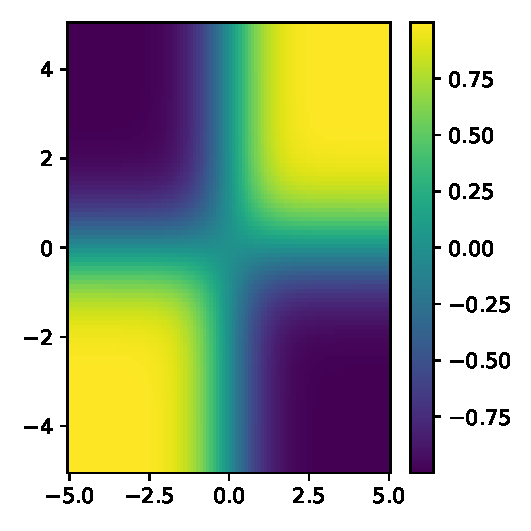
\includegraphics[width = \textwidth]{plots/weight_by_probability.pdf}
		\caption{Gewichtung mit der Wahrscheinlichkeit eines normalverteilten Messfehlers für $\sigma = 1$}
  		\label{fig:weighting}	
  	\end{subfigure}
	\begin{subfigure}{.48\textwidth}
  		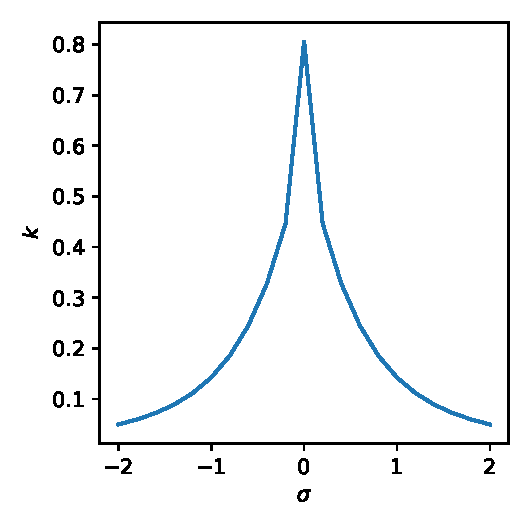
\includegraphics[width=\textwidth]{plots/mean_k_over_sigma.pdf}
  		\caption{Mittleres $k$ über $1000$ Realisierungen in Abhängigkeit von $\sigma$.}
	\end{subfigure}
	\caption{Plots zum Maß $k$.}
  	\label{fig:k}
\end{figure}

\subsection{Wie könnte man $\sigma$ bestimmen?}

Vermutung: Wenn man $\bar{k}(z_b)$ für gegebenen Vektor $z_b^1, \dots$ für verschiedene $\sigma$ berechnet, hat $\bar{k}(z_b)$ beim "echten" $\sigma$ einen Wendepunkt.

Ist im Umkehrschluss die Vorgehensweise oben eine Möglichkeit, Rauschen in den Daten zu bestimmen?

\subsection{Alternative Vorgehensweise}
Die Formel (\ref{eq:concordance}) ist eine einfache und effiziente Methode zur Messung der Konkordanz, aber die Effektivität nimmt schnell ab, wenn die Daten verrauscht sind. Daher liegt es nahe, die verwendeten Daten zunächst zu entrauschen, bevor ein Trendfähigkeitsmaß auf sie angewendet wird. 

Ob und wie stark die Schätzung eines Nowcasters verrauscht ist, ist eine Eigenschaft des Nowcasters. Starkes Rauschen bedeutet, dass der Schätzer nicht robust ist. Es ist daher nicht notwendig, die Werte des Nowcasters zu entrauschen. Die realen Daten der zu schätzenden Größe sollten jedoch mit einer geeigneten Technik entrauscht werden oder die Verteilungsinformation des Rauschens (z. B. in Form einer Normalfehlerverteilung) sollte aus den Daten gelernt werden. Die entrauschten Daten bzw. die allgemeine Verteilung des wahren Wertes sollten dann mit dem (angepassten) Maß weiterverarbeitet werden. Ein Ablaufschema ist in Abb. \ref{fig:ablauf} dargestellt.

\begin{figure}
    \centering
    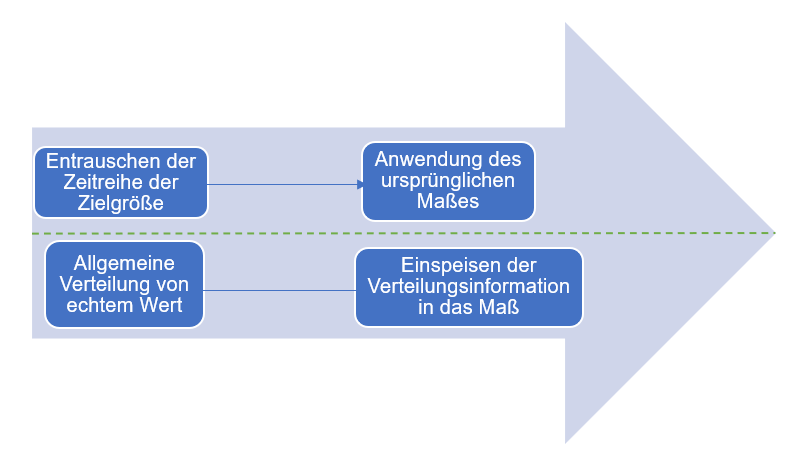
\includegraphics[width=1\linewidth]{plots/ablauf.png}
    \caption{Alternativer Ablaufplan}
    \label{fig:ablauf}
\end{figure}

Hier seien ein paar Standardmethoden in der Literatur genannt,die das Entrauschen betreffen. 

\begin{itemize}
    \item Domänwissen
    \item Glättungstechniken
    \item Frequenzenanalyse
\end{itemize}

Schließlich wird noch diskutiert, inwieweit es sinnvoll ist, die Ergebnisse verschiedener Lags zu kombinieren.

Die Bedeutung des Lags hängt von der konkreten Anwendung ab. Es könnte daher sinnvoll sein, eine Methodik zu definieren, die auf der Grundlage subjektiver Einschätzungen Gewichtungen für die einzelnen Lags liefert.

\subsection{Gewichtete Konkordanz-Formel}

Motivation

\begin{itemize}
    \item Bei einer signifikanten Zunahme/Abnahme des tatsächlichen Wertes wird auch der Wert des Nowcaster-Schätzers signifikant erhöht/verringert.
    \item Signifikanz gemessen an dem aktuellen tatsächlichen Wert
    \item mind. so siginifikant heißt, mind. gleich viel relative Änderung wird vorhergesagt
    \item In solchem Fall sollte eine Vorhersage in die falsche Richtung im Bezug auf Trendability strenger bestraft werden.
    \item Betrachtung der relativen Änderung (immer im Bezug auf $\max{Y_t, Y_{t+1}}$)
    \item Gewicht der Konkordanz proportinal zu dem Betrag der relativen Änderung.
\end{itemize}

Diese Überlegungen führen zu folgedem Formelvorschlag (für Lag = 1): 
\[\lag X_t = X_{t+1}-Y_{t}\]
\[\lag Y_t = Y_{t+1}-Y_{t}\]

Berechnung der Gewichtung: 
\[w_t=\frac{\abs{\lag Y_t}}{\sum_{k=1}^{T-1}\abs{\lag Y_k}}\]

Relative Veränderungen:
\[\delta Y_t = \frac{\lag Y_t}{\min\{Y_t, Y_{t+1}\}} \]
\[\delta X_t = \frac{\lag X_t}{\min\{Y_t, X_{t+1}\}} \]

Gewichtete Formel
\begin{equation}
  \sum_{t = 1}^{T - 1} w_t \max\{\min\{\frac{\delta X_t}{\delta Y_t},1\},0\}
\end{equation}

\subsection{Weiterentwicklung der Methodik}


\section{Erste Simulationsstudie}
\begin{itemize}
    \item $\lag Y_t \sim \mathcal{N}$
    \item $X_t = X_{t-1} + \abs{Z} (2 (U < k) - 1) \sign(Y_t - Y_{t-1})$ ($Z \sim \mathcal{N}, U \sim \mathcal{U}(0, 1)$) \todo{Rückkopplung an $Y_{t-1}$}
    \item $X_t = Y_{t-1} + \abs{Z} (2 (U < k) - 1) \sign(Y_t - Y_{t-1})$ ($Z \sim \mathcal{N}, U \sim \mathcal{U}(0, 1)$)
\end{itemize}



%\subsection{Modellierung}
%\begin{itemize}
%  \item Sei $l$ der zeitliche Abstand, mit dem Realisationen verfügbar werden
%  \item $Y_{t + l} = Y_t + \lag Y_t$
%  \item Die Nowcast schätzen (fehlerbehaftet) $\lag Y_t$ mithilfe von Daten, die zum Zeitpunkt $\tau \in T_t^k$ verfügbar sind, und dem neuesten, bekannten Wert $Y_t$:
%	\begin{equation}
%  		X_{t \lvert \tau}^k = Y_{\tau - l} + (\widehat{\lag[t-\tau+l] Y_t})_{t \lvert \tau}^k,
%	\end{equation}
%	wobei
%		\begin{equation}
%  			\lag[t-\tau+l] Y_t =  (\widehat{\lag[t-\tau+l] Y_t})_{t \lvert \tau}^k + \varepsilon.
%		\end{equation}


%\end{itemize}
\section{Weitere Ideen zu Trending}

\begin{itemize}
  \item \enquote{Schwaches} Trending für lag $l$: Wahrscheinlichkeit, in die gleiche Richtung zu zeigen ist größer als Wahrscheinlichkeit in die falsche Richtung zu zeigen (für lag $l$)
  \item \enquote{Downwards}-Trending: Trends in die negative Richtung werden erkannt, in die positive Richtung nicht
  \item \enquote{Upwards}-Trending: Trends in die positive Richtung werden erkannt, in die negative nicht
  \item Nicht einfach nur 0-1-Kodierung für gleiches Vorzeichen von $\lag x$ und $\lag y$, sondern Gewichtung des $\mathbb{R}^2$, sodass zum Beispiel Punkte nahe der Achsen weniger Gewicht bekommen als solche nahe der Winkelhalbierenden
  \item PCA auf $\lag x$ und $\lag y$, Bestrafung der zweiten Komponente (Abweichung von Gerade): Bestrafung würde aber mehr umfassen, als lediglich den Trend, sondern würde Abweichung von Linearität betreffen
  \item Falls wir Exclusion Area wollen und $\lag Y_t$ heteroskedastisch: relative Werte betrachten?
\end{itemize}

%\printbibliography

\begin{comment}

Gegeben sind zwei Zeitreihen $(x_t)$ und $(y_t)$, $t\in \{t_0,...,t_N\}$. Dabei kann $(x_t)$ die zeitliche Entwicklung einer Zielgröße und $(y_t)$ die zeitlichen Schätzungen eines Nowcasters darstellen. Uns interessiert, ob die Entwicklungen der beiden Zeitreihen den gleichen Trend aufweisen bzw. ob der Nowcaster die Entwicklung der zu schätzenden Größe mit dem richtigen Trend schätzen kann. Es sollte ein Maß konstruiert werden, das beschreibt, wie gut zwei Zeitreihen den gleichen Trend aufweisen.

\subsection{Anforderungen an einem Maß/ Intuitionen}

Zwei Zeitreihen weisen den gleichen Trend auf, wenn für zwei beliebige Zeitpunkte $t$ und $\tau$ gilt: $(x_t-x_\tau)(y_t-y_\tau)>0$ oder $x_t=x_\tau \land y_t = y_\tau$.

\todo{Kann man theoretisch nicht einfach mit Rang-korrelations-koeffizient Trending überprüfen?}
\subsection{Ein einfaches Maß}
Sei $\Delta_{t,\tau}^{x}:=x_\tau-x_t$.
\begin{equation}
  		R_{t,\tau}^{x,y} \coloneqq 
        \begin{cases}
  		    \frac{\Delta_{t,\tau}^{x}\Delta_{t,\tau}^{y}}   {\vert\Delta_{t,\tau}^{x}\vert\vert\Delta_{t,\tau}^{y}\vert } &, \text{falls} \Delta_{t,\tau}^{x}\neq 0 \land \Delta_{t,\tau}^{y}\neq0\\
           1 &, \text{falls} \Delta_{t,\tau}^{x}=\Delta_{t,\tau}^{y}=0\\
            -1 &, \text{sonst} 
  	\end{cases}
	\end{equation}
Beispiel-Maß: $S(\bold{x},\bold{y})=\sum_{k=1}^{k^*}\frac{w_k}{N+1-k}\sum_{j=0}^{N-k}R_{t_j,t_{j+k}}^{x,y},$
wobei $w_k, k=1,...,k^*$ eine Gewichtung für das Trending-Verhalten in verschiedenen Zeitdistanzen darstellt. Dabei erfüllt $w_k$ die folgenden Anforderungen:

\begin{itemize}
    \item $w_k$ ist streng monoton fallend in $k$. Hintergrund: je klein der betrachtete Zeitabstand ist, desto größer ist hier der Einfluss des Rauschens
    \item $\sum_{k=1}^{k^*}w_k=1$
\end{itemize}

\subsection{Eigenschaften des vorgeschlagenen Maßes}
\begin{itemize}
    \item Seien $(x_n)$ und $(y_n)$ zwei Realisierungen eines Random Walk -Modells.\\
    Hypothese: $S((x_n),(y_n))=0$. \\
    Intuition:  Zwei Random Walks $(x_n)$ und $(y_n)$ zeigen kein gemeinsames Tendenzverhalten auf. 
\end{itemize}

\subsection{Gewichtung für das Maß $k$}

Idee: Man betrachtet für jeden Punkt $(\lag x, \lag y)$ die Wahrscheinlichkeit für diesen Punkt in jedem der vier Quadranten zu liegen, wenn Messfehler abgezogen werden.
Dann gewichten wir das Maß 
\begin{equation}
    k (x, y; l, \epsilon) = \frac{\sum_{t}^{n-l}  \omega k^s (\lag y_t, \lag x_t; l, \epsilon)}{\sum_{t}^{n-l} k^\epsilon (\lag y_t, \lag x_t)},
\end{equation}
mit $\omega = P(Q_{ru}) + P(Q_{ll}) - P(Q_{lu}) - P(Q_{rl})$ für jeden Punkt. \todo{$\omega$ ist Funktion von jedem Punkt (siehe Blatt)}


Gewichtung über verschiedene lags entweder optimieren oder über Plots verschiedene Lags darstellen
 

% \section{Statistische Modellierung}
% \subsection{Modellierung}
% \begin{itemize}
%   \item Sei $l$ der zeitliche Abstand, mit dem Realisationen verfügbar werden
%   \item $Y_{t + l} = Y_t + \lag Y_t$
%   \item Die Nowcast schätzen (fehlerbehaftet) $\lag Y_t$ mithilfe von Daten, die zum Zeitpunkt $\tau \in T_t^k$ verfügbar sind, und dem neuesten, bekannten Wert $Y_t$:
% 	\begin{equation}
%   		X_{t \lvert \tau}^k = Y_{\tau - l} + (\widehat{\lag[t-\tau+l] Y_t})_{t \lvert \tau}^k,
% 	\end{equation}
% 	wobei
% 		\begin{equation}
%   			\lag[t-\tau+l] Y_t =  (\widehat{\lag[t-\tau+l] Y_t})_{t \lvert \tau}^k + \varepsilon.
% 		\end{equation}


<<<<<<< Updated upstream
% \end{itemize}
\subsection{Weitere Ideen zu Trending}

\begin{itemize}
  \item \enquote{Schwaches} Trending für lag $l$: Wahrscheinlichkeit, in die gleiche Richtung zu zeigen ist größer als Wahrscheinlichkeit in die falsche Richtung zu zeigen (für lag $l$)
  \item \enquote{Downwards}-Trending: Trends in die negative Richtung werden erkannt, in die positive Richtung nicht
  \item \enquote{Upwards}-Trending: Trends in die positive Richtung werden erkannt, in die negative nicht
  \item \enquote{Complete}-Trending: Trends in beiden Richtungen werden erkannt
  \item Nicht einfach nur 0-1-Kodierung für gleiches Vorzeichen von $\lag x$ und $\lag y$, sondern Gewichtung des $\mathbb{R}^2$, sodass zum Beispiel Punkte nahe der Achsen weniger Gewicht bekommen als solche nahe der Winkelhalbierenden
  \item PCA auf $\lag x$ und $\lag y$, Bestrafung der zweiten Komponente (Abweichung von Gerade): Bestrafung würde aber mehr umfassen, als lediglich den Trend, sondern würde Abweichung von Linearität betreffen
  \item Falls wir Exclusion Area wollen und $\lag Y_t$ heteroskedastisch: relative Werte betrachten?
\end{itemize}

\section{Simulationsstudie}

\begin{itemize}
    \item $\lag Y_t \sim \mathcal{N}$
    \item $X_t = X_{t-1} + \abs{Z} (2 (U < k) - 1) \sign(Y_t - Y_{t-1})$ ($Z \sim \mathcal{N}, U \sim \mathcal{U}(0, 1)$) \todo{Rückkopplung an $Y_{t-1}$}
    \item $X_t = Y_{t-1} + \abs{Z} (2 (U < k) - 1) \sign(Y_t - Y_{t-1})$ ($Z \sim \mathcal{N}, U \sim \mathcal{U}(0, 1)$)
\end{itemize}

%\printbibliography


||||||| Stash base

\section{Statistische Modellierung}
\subsection{Modellierung}
\begin{itemize}
  \item Sei $l$ der zeitliche Abstand, mit dem Realisationen verfügbar werden
  \item $Y_{t + l} = Y_t + \lag Y_t$
  \item Die Nowcast schätzen (fehlerbehaftet) $\lag Y_t$ mithilfe von Daten, die zum Zeitpunkt $\tau \in T_t^k$ verfügbar sind, und dem neuesten, bekannten Wert $Y_t$:
	\begin{equation}
  		X_{t \lvert \tau}^k = Y_{\tau - l} + (\widehat{\lag[t-\tau+l] Y_t})_{t \lvert \tau}^k,
	\end{equation}
	wobei
		\begin{equation}
  			\lag[t-\tau+l] Y_t =  (\widehat{\lag[t-\tau+l] Y_t})_{t \lvert \tau}^k + \varepsilon.
		\end{equation}


\end{itemize}
\subsection{Weitere Ideen zu Trending}

\begin{itemize}
  \item \enquote{Schwaches} Trending für lag $l$: Wahrscheinlichkeit, in die gleiche Richtung zu zeigen ist größer als Wahrscheinlichkeit in die falsche Richtung zu zeigen (für lag $l$)
  \item \enquote{Downwards}-Trending: Trends in die negative Richtung werden erkannt, in die positive Richtung nicht
  \item \enquote{Upwards}-Trending: Trends in die positive Richtung werden erkannt, in die negative nicht
  \item Nicht einfach nur 0-1-Kodierung für gleiches Vorzeichen von $\lag x$ und $\lag y$, sondern Gewichtung des $\mathbb{R}^2$, sodass zum Beispiel Punkte nahe der Achsen weniger Gewicht bekommen als solche nahe der Winkelhalbierenden
  \item PCA auf $\lag x$ und $\lag y$, Bestrafung der zweiten Komponente (Abweichung von Gerade): Bestrafung würde aber mehr umfassen, als lediglich den Trend, sondern würde Abweichung von Linearität betreffen
  \item Falls wir Exclusion Area wollen und $\lag Y_t$ heteroskedastisch: relative Werte betrachten?
\end{itemize}

%\printbibliography


\end{comment}

\end{document} 